% lint-skip: 未完成ステータス（figure/table caption 未対応，人手チェック時に解消予定）
\documentclass[../../main.tex]{subfiles}
\begin{document}

\begin{flushright}
  \footnotesize\textit{【自動文字起こし・要確認】}
\end{flushright}

[解] (1) $P(t, 4-t^2)$ とおく. ($-4 \le t \le 1$)
$\triangle PAB = \dfrac{1}{2} |AB| \cdot (P \text{と} AB \text{のキョリ})$
だから, $P$ と $AB$ のキョリ $l$ が最大の時, $\triangle PAB$ の面積も最大.
\begin{figure}[htb]
  \centering
  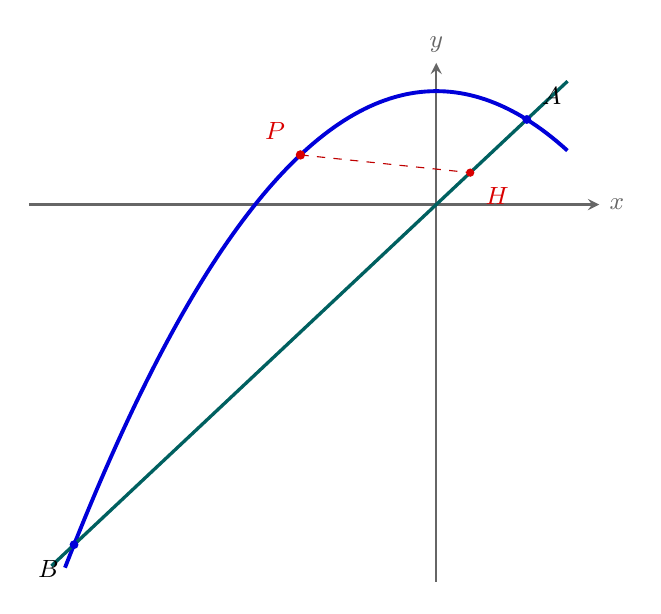
\begin{tikzpicture}[x=1.15cm, y=0.36cm, >=stealth,
    every node/.style={font=\small}]
    \coordinate (A) at (1,3);
    \coordinate (B) at (-4,-12);
    \coordinate (P) at (-1.5,1.75);
    \coordinate (H) at (0.375,1.125);
    \draw[->, thick, gray!80!black] (-4.5,0) -- (1.8,0) node[right] {$x$};
    \draw[->, thick, gray!80!black] (0,-13.3) -- (0,5) node[above] {$y$};
    \draw[line width=1.4pt, blue!85!black, domain=-4.1:1.45, samples=100]
    plot (\x,{4-\x*\x});
    \draw[line width=1.2pt, teal!75!black] (-4.25,-12.75) -- (1.45,4.35);
    \draw[dashed, red!75!black] (P) -- (H);
    \foreach \X in {A,B} {\fill[blue!85!black] (\X) circle (1.6pt);}
    \fill[red!85!black] (P) circle (1.7pt);
    \fill[red!85!black] (H) circle (1.5pt);
    \node[above right=2pt] at (A) {$A$};
    \node[below left=2pt] at (B) {$B$};
    \node[above left=2pt, red!85!black] at (P) {$P$};
    \node[below right=2pt, red!85!black] at (H) {$H$};
  \end{tikzpicture}
  \caption{放物線 $y=4-x^2$ 上の点 $P$ から直線 $AB:y=3x$ までの距離 $PH$}
\end{figure}
\[ l = \dfrac{|3t - (4-t^2)|}{\sqrt{9+1}} = \dfrac{|t^2 + 3t - 4|}{\sqrt{10}} = \dfrac{\sqrt{10}}{10} \left| \left(t+\dfrac{3}{2}\right)^2 - \dfrac{25}{4} \right| \]
より, $\max l = \dfrac{\sqrt{10}}{10} \cdot \dfrac{25}{4}$ ($t = -\dfrac{3}{2}$ の時) だから
もとめる $P(p, q)$ は $P\left(-\dfrac{3}{2}, \dfrac{7}{4}\right)$ \qed
\begin{figure}[htb]
  \centering
  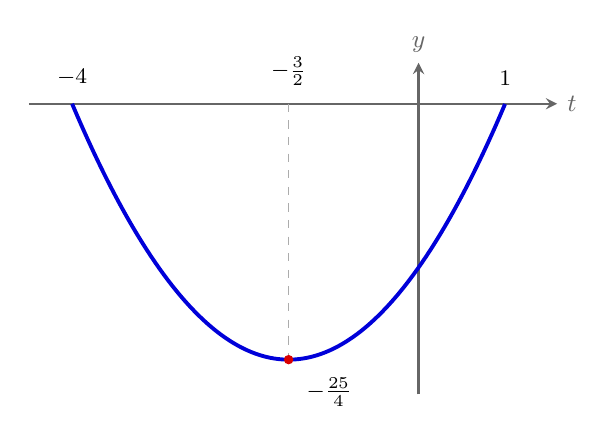
\begin{tikzpicture}[x=1.1cm, y=0.52cm, >=stealth,
    every node/.style={font=\small}]
    \draw[->, thick, gray!80!black] (-4.5,0) -- (1.6,0) node[right] {$t$};
    \draw[->, thick, gray!80!black] (0,-7.1) -- (0,1.0) node[above] {$y$};
    \draw[line width=1.4pt, blue!85!black, domain=-4:1, samples=100]
    plot (\x,{(\x+1.5)*(\x+1.5)-6.25});
    \draw[dashed, gray!65] (-1.5,0) -- (-1.5,-6.25);
    \fill[red!85!black] (-1.5,-6.25) circle (1.7pt);
    \node[above=3pt, font=\footnotesize] at (-4,0) {$-4$};
    \node[above=3pt, font=\footnotesize] at (1,0) {$1$};
    \node[above=3pt, font=\footnotesize] at (-1.5,0) {$-\frac32$};
    \node[below right=3pt, font=\footnotesize] at (-1.5,-6.25)
    {$-\frac{25}{4}$};
  \end{tikzpicture}
  \caption{$t^2+3t-4$ は $t=-3/2$ で最小となり，距離が最大となる}
\end{figure}

\paragraph{(2)}

題意の直線は $y = 3x + \alpha$ とおける ($\alpha \in \mathbb{R}$). これと放物線の交点の $x$ 座標は
\[ x^2 + 3x + \alpha - 4 = 0 \]
の2解であり, $x = \dfrac{1}{2}\left(-3 \pm \sqrt{25 - 4\alpha}\right)$ だから, $CD$ の中点 $M$ の
$x$ 座標は $x = -\dfrac{3}{2}$ となる. したがって(1)から, 線分 $CD$ は $x = p$ で
2等分される. \qed

\paragraph{(3)}

右図のように面積をおく ($S = S_1 + S_2$)
\[ S = \int_{-4}^{1} (4 - x^2 - 3x) dx = \dfrac{1}{6} 5^3 \]
\[ S_1 = \int_{-4}^{-\frac{3}{2}} (4 - x^2 - 3x) dx = -\dfrac{1}{3}\left(\dfrac{5}{2}\right)^3 + \dfrac{5}{2}\left(\dfrac{5}{2}\right)^2 = \dfrac{1}{12} 5^3 \]
よって $S_1 = S_2$ となるから示された \qed

\begin{figure}[htb]
  \centering
  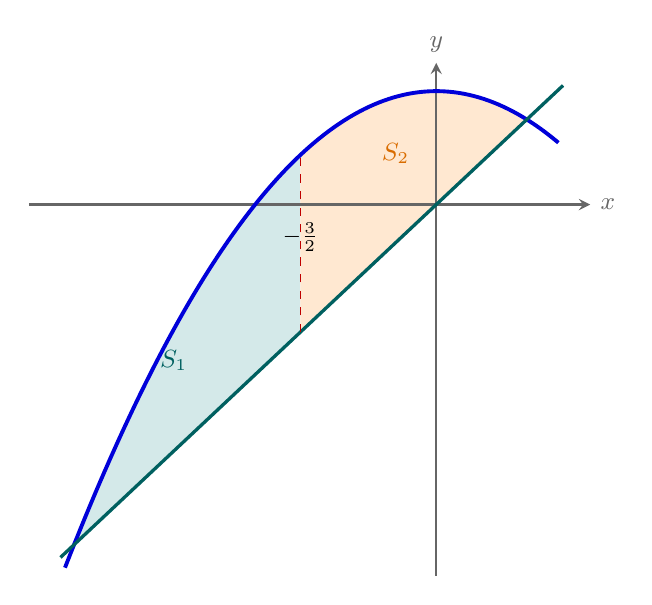
\begin{tikzpicture}[x=1.15cm, y=0.36cm, >=stealth,
    every node/.style={font=\small}]
    \fill[teal!17] plot[domain=-4:-1.5,samples=65] (\x,{4-\x*\x})
    -- plot[domain=-1.5:-4,samples=65] (\x,{3*\x}) -- cycle;
    \fill[orange!18] plot[domain=-1.5:1,samples=65] (\x,{4-\x*\x})
    -- plot[domain=1:-1.5,samples=65] (\x,{3*\x}) -- cycle;
    \draw[->, thick, gray!80!black] (-4.5,0) -- (1.7,0) node[right] {$x$};
    \draw[->, thick, gray!80!black] (0,-13.1) -- (0,5) node[above] {$y$};
    \draw[line width=1.4pt, blue!85!black, domain=-4.1:1.35, samples=100]
    plot (\x,{4-\x*\x});
    \draw[line width=1.2pt, teal!75!black] (-4.15,-12.45) -- (1.4,4.2);
    \draw[dashed, red!75!black] (-1.5,-4.5) -- (-1.5,1.75);
    \node[below=3pt, font=\footnotesize] at (-1.5,0) {$-\frac32$};
    \node[teal!75!black] at (-2.9,-5.5) {$S_1$};
    \node[orange!85!black] at (-0.45,1.8) {$S_2$};
  \end{tikzpicture}
  \caption{直線 $x=-3/2$ で分けた2領域 $S_1$ と $S_2$}
\end{figure}

\end{document}
